% !TEX TS-program = XeLaTeX
% use the following command:
% all document files must be coded in UTF-8
\documentclass[portuguese]{textolivre}
% build HTML with: make4ht -e build.lua -c textolivre.cfg -x -u article "fn-in,svg,pic-align"

\journalname{Texto Livre}
\thevolume{17}
%\thenumber{1} % old template
\theyear{2024}
\receiveddate{\DTMdisplaydate{2023}{6}{27}{-1}}
\accepteddate{\DTMdisplaydate{2023}{10}{22}{-1}}
\publisheddate{\DTMdisplaydate{2024}{1}{4}{-1}}
\corrauthor{Lilian Karla Rocha}
\articledoi{10.1590/1983-3652.2024.46657}
%\articleid{NNNN} % if the article ID is not the last 5 numbers of its DOI, provide it using \articleid{} commmand 
% list of available sesscions in the journal: articles, dossier, reports, essays, reviews, interviews, editorial
\articlesessionname{articles}
\runningauthor{Rocha e Ribeiro}
%\editorname{Leonardo Araújo} % old template
\sectioneditorname{Bárbara Amaral da Silva}
\layouteditorname{Daniervelin Pereira}

\title{Os imaginários sociodiscursivos do ensino de escrita da redação do Enem de influenciadores digitais}
\othertitle{Sociodiscursive imaginaries of digital influencers in the writing teaching for the brazilian national secondary education examination (Enem)}
% if there is a third language title, add here:
%\othertitle{Artikelvorlage zur Einreichung beim Texto Livre Journal}

\author[1]{Lilian Karla Rocha~\orcid{0000-0003-3517-1267}\thanks{Email: \href{mailto:lilian.karla.rocha@educacao.mg.gov.br}{lilian.karla.rocha@educacao.mg.gov.br}}}
\author[2]{Maria Clara Maciel de Araújo Ribeiro~\orcid{0000-0001-9205-5858}\thanks{Email: \href{mailto:maria.ribeiro@unimontes.br}{maria.ribeiro@unimontes.br}}}\affil[1]{Universidade Estadual de Montes Claros, Programa de pós-graduação em Educação, Montes Claros, MG, Brasil.}
\affil[2]{Universidade Estadual de Montes Claros, Departamento de Comunicação e Letras, Montes Claros, MG, Brasil.}


\addbibresource{article.bib}
% use biber instead of bibtex
% $ biber article

% used to create dummy text for the template file
\definecolor{dark-gray}{gray}{0.35} % color used to display dummy texts
\usepackage{lipsum}
\SetLipsumParListSurrounders{\colorlet{oldcolor}{.}\color{dark-gray}}{\color{oldcolor}}

% used here only to provide the XeLaTeX and BibTeX logos
\usepackage{hologo}

% if you use multirows in a table, include the multirow package
\usepackage{multirow}

% provides sidewaysfigure environment
\usepackage{rotating}

% CUSTOM EPIGRAPH - BEGIN 
%%% https://tex.stackexchange.com/questions/193178/specific-epigraph-style
\usepackage{epigraph}
\renewcommand\textflush{flushright}
\makeatletter
\newlength\epitextskip
\pretocmd{\@epitext}{\em}{}{}
\apptocmd{\@epitext}{\em}{}{}
\patchcmd{\epigraph}{\@epitext{#1}\\}{\@epitext{#1}\\[\epitextskip]}{}{}
\makeatother
\setlength\epigraphrule{0pt}
\setlength\epitextskip{0.5ex}
\setlength\epigraphwidth{.7\textwidth}
% CUSTOM EPIGRAPH - END

% LANGUAGE - BEGIN
% ARABIC
% for languages that use special fonts, you must provide the typeface that will be used
% \setotherlanguage{arabic}
% \newfontfamily\arabicfont[Script=Arabic]{Amiri}
% \newfontfamily\arabicfontsf[Script=Arabic]{Amiri}
% \newfontfamily\arabicfonttt[Script=Arabic]{Amiri}
%
% in the article, to add arabic text use: \textlang{arabic}{ ... }
%
% RUSSIAN
% for russian text we also need to define fonts with support for Cyrillic script
% \usepackage{fontspec}
% \setotherlanguage{russian}
% \newfontfamily\cyrillicfont{Times New Roman}
% \newfontfamily\cyrillicfontsf{Times New Roman}[Script=Cyrillic]
% \newfontfamily\cyrillicfonttt{Times New Roman}[Script=Cyrillic]
%
% in the text use \begin{russian} ... \end{russian}
% LANGUAGE - END

% EMOJIS - BEGIN
% to use emoticons in your manuscript
% https://stackoverflow.com/questions/190145/how-to-insert-emoticons-in-latex/57076064
% using font Symbola, which has full support
% the font may be downloaded at:
% https://dn-works.com/ufas/
% add to preamble:
% \newfontfamily\Symbola{Symbola}
% in the text use:
% {\Symbola 😥}
% EMOJIS - END

% LABEL REFERENCE TO DESCRIPTIVE LIST - BEGIN
% reference itens in a descriptive list using their labels instead of numbers
% insert the code below in the preambule:
%\makeatletter
%\let\orgdescriptionlabel\descriptionlabel
%\renewcommand*{\descriptionlabel}[1]{%
%  \let\orglabel\label
%  \let\label\@gobble
%  \phantomsection
%  \edef\@currentlabel{#1\unskip}%
%  \let\label\orglabel
%  \orgdescriptionlabel{#1}%
%}
%\makeatother
%
% in your document, use as illustraded here:
%\begin{description}
%  \item[first\label{itm1}] this is only an example;
%  % ...  add more items
%\end{description}
% LABEL REFERENCE TO DESCRIPTIVE LIST - END


% add line numbers for submission
%\usepackage{lineno}
%\linenumbers

\begin{document}
\maketitle

\begin{polyabstract}
\begin{abstract}
O avanço tecnológico proporcionou a criação de novos espaços de divulgação do conhecimento. Logo, discursos voltados para o ensino de escrita começaram a circular em plataformas digitais com o intuito de propagar conhecimentos relativos à escrita da redação do Enem. A partir disso, o objetivo deste estudo é delinear os imaginários sociodiscursivos que alicerçam o ensino de escrita da redação do Enem de influenciadores digitais, considerando a oferta da aprendizagem como uma mercadoria cultural. Para isso, utiliza-se uma abordagem qualitativa e explicativa, baseando-se na Análise do Discurso, de perspectiva francesa, sobretudo a partir de \textcite{charaudeau_os_2017}, com contribuições pontuais da teoria crítica. Como corpus, foram selecionados três vídeos, tendo como critério as maiores visualizações no YouTube e a palavra-chave de busca: “redação Enem”. As análises apontam para uma movimentação de saberes de conhecimento que, ao serem tecidos, misturam a teoria sobre escrita de textos dissertativos com o manual do Inep e com as experiências próprias de cada influenciador com a prova discursiva do Enem. Esta proposta vaga de ensino de escrita revela uma objetificação do ato de escrever, transformando-o em produto a ser comercializado na medida em que, a partir da empiria, os influenciadores demonstram sucesso próprio no Enem.

\keywords{Imaginários sociodiscursivos \sep Redação do Enem \sep Ensino de escrita \sep Mercadoria \sep Influenciadores digitais}
\end{abstract}

\begin{english}
\begin{abstract}
Technological advances have given rise to the creation of new spaces for the dissemination of knowledge. Thus, discourses regarding the teaching of writing began to circulate on digital platforms in order to propagate knowledge related to the writing of the Enem essay. Having this in mind, the aim of this study is to delineate the sociodiscursive imaginaries that underpin digital influencers' teaching of Enem essay writing, considering the offer of the learning process as a cultural commodity. For this purpose, a qualitative and explanatory approach is used, based on Discourse Analysis from French perspective, mostly based on \textcite{charaudeau_os_2017}, with contributions from the concept of Cultural Commodity from Critical Theory. As a corpus, three videos were selected, using as criteria the largest number of views on YouTube and the search keyword "redação Enem" (Enem essay). The analyses point to a movement of expertise-related knowledge that, when woven, mixes the theory on writing discursive texts with the Inep manual, as well as with each influencer's own experiences with the Enem discursive test. This vague proposal for teaching writing reveals an objectification of the act of writing, transforming it into a product to be marketed to the extent that, from empirical experience, influencers demonstrate their own success in the Enem test.

\keywords{Sociodiscursive imaginaries \sep Enem essay \sep Teaching of writing \sep Commodity \sep Digital influencers}
\end{abstract}
\end{english}
% if there is another abstract, insert it here using the same scheme
\end{polyabstract}


\section{Introdução}
A linguagem medeia relações humanas, e tecnologias digitais, hoje, medeiam a própria relação do homem com a linguagem. Com a internet, interações tornaram-se instantâneas e massificadas, possibilitando a criação de espaços virtuais que conectam um sem-número de pessoas. A partir disso, vozes formativas já não são ecoadas apenas pela escola, devido à imensa disseminação de conhecimentos que se processa pela internet, mas também pelas mídias sociais, que se utilizam de linguagem simplificada e conteúdo esquematizado, cooptando um público amplo e diversificado que busca entretenimento informativo. 

Há uma máxima que diz que depois dos tutoriais do \textit{Youtube} até um leigo faz uma cirurgia cardíaca, desde que siga um passo a passo. Apesar de exagerado, o enunciado alude à capacidade das mídias sociais ensinarem, com relativo sucesso, muitas coisas, entre elas, processos de escrita, como a elaboração da redação do Enem – gênero textual definidor do acesso (ou não) de estudantes ao Ensino Superior público, dado o peso desta que é a única prova aberta do exame\footnote{A redação vale 1000 pontos, assim como cada uma das quatro áreas do conhecimento, equivalendo então 1/5 da nota total.}.

Nota-se que é sobretudo dentro da escola que os discursos sobre redação do Enem se formam, mas é por meio da internet que eles se difundem e se transformam amplamente, midiatizando conteúdos educacionais antes limitados ao âmbito institucional. É nessa perspectiva que influenciadores digitais\footnote{Profissional do marketing de influência que cria \textbf{conteúdo} para mídias sociais com o intuito de \textbf{atrair um público} a ser influenciado.} disseminam conteúdos de maneira “fácil”, objetiva, fragmentada e descontraída, a fim de buscar engajamento\footnote{É a participação ativa e voluntária a um determinado conteúdo disseminado por um influenciador.} de seus seguidores/espectadores e de diferenciar-se do padrão escola de difusão de conhecimento.

Embora certas redes de ensino privado abordem o ensino da redação do Enem em moldes semelhantes, entende-se que o alcance delas seja limitado por aspectos espaço-temporais, enquanto a projeção de influenciadores em redes virtuais torna a extensão deste alcance quase incalculável. Este alcance revela uma espécie de midiatização de conteúdos escolares que transforma o próprio conhecimento em um produto de consumo fácil que irá atender aos anseios de jovens que buscam uma vaga na universidade. A partir desse cenário surge o questionamento: o que significa ensinar a escrever para esses influenciadores digitais? Como eles projetam para si e para os outros este fazer? 

A partir dessas questões, este artigo objetiva delinear os imaginários sociodiscursivos que alicerçam o ensino de escrita da redação Enem de influenciadores digitais com canais na plataforma Youtube\footnote{Plataforma escolhida por ser o mais importante meio de divulgação de vídeos \textit{online}, além alcançar um público abrangente.}. Para tanto, serão selecionados vídeos de influenciadores que atuam sobre o tema “redação do Enem” na plataforma. O critério de seleção relaciona-se à escolha de vídeos com grandes números de visualização.

Assim, na plataforma, foram realizadas buscas a partir dos termos “redação + Enem” e os três vídeos com maior número de visualização (em fevereiro de 2022) foram selecionados. Para analisar os dados, parte-se da Análise do Discurso de tendência francesa, representada por \textcite{charaudeau_os_2017,charaudeau_discurso_2018} e Dominique \textcite{maingueneau_proposito_2008,maingueneau_analise_2012}, com diálogos precisos com a teoria crítica. 

Para o desdobramento da proposta, desenvolve-se, inicialmente, uma discussão histórica sobre o ensino de escrita, o conceito de imaginários sociodiscursivos e a figura de influenciadores digitais. Posteriormente, apresentam-se os procedimentos metodológicos da pesquisa e, por fim, focalizam-se discursos de influenciadores digitais, encaminhando o artigo para as conclusões.

\section{Para contextualizar o ensino de escrita da redação do ENEM}\label{sec-normas}
Na perspectiva que assumimos, o ato de ensinar não é meramente transferir o que o educador sabe, mas permitir ao educando refletir sobre aquilo que ele lê, escuta e produz \cite{freire_pedagogia_1996}.

Todavia, a rigor, o processo de ensino-aprendizagem da escrita da redação do ENEM utiliza-se de modelos textuais pré-formatados, que devem ser reproduzidos fielmente pelos estudantes. Por um lado, essa prática é reflexo da herança deixada pelos séculos XVIII até meados do século XX, que concebiam o ensino da escrita enquanto (de)codificação e uso de regras gramaticais memorizadas \cite{bunzen_da_2006}. Por outro, entende-se que os critérios de avaliação da redação instituídos pelo INEP vão empurrando os professores a processos de ensino cada vez menos dialógicos e mais padronizados.  

\textcite{bonini_metodologias_2002} explica que o “bem-escrever” foi pautado em um método retórico-lógico que não permitia sair da “bolha” criada pelo binômio leitura/gramática instituído e disseminado no século XVIII. Assim, nos anos de 1960, nas escolas brasileiras, esse método ditava a “organização do pensamento” e, com isso, o processo de escrita nada mais era do que a repetição de “estruturas” aliadas ao conhecimento de regras gramaticais. Desse modo, não se educava para o uso autônomo da linguagem, mas para uma mera repetição esvaziada de reflexão, o que revela a forte influência de uma perspectiva de educação bancária no ensino de linguagem, como alertava \textcite{freire_pedagogia_1996}. 

Inovações legislativas de amparo ao abandono do modelo retórico-lógico começaram a surgir na década de 1960, estando também embasadas na primeira Lei de Diretrizes e Bases da educação \cite{brasil_lei_1961}. Mas embora se observem algumas modificações no discurso oficial, incluindo o aumento da maleabilidade dos currículos básicos e instruções para a elaboração de materiais didáticos, observa-se que o tripé leitura-redação-gramática manteve-se forte, permanecendo como a base dos processos de ensino de linguagem.  

Em seguida, as teorias da comunicação nos anos de 1970 e a Lei 5.692 de 1971, que orientava sobre as Diretrizes e Bases para o ensino do chamado 1° e 2º graus, associadas, buscavam preparar o discente para o trabalho, ou seja, estar apto a exercer uma determinada função laboral \cite{vicentini_redaco_2015}. Entretanto, mesmo que tenham sido realizados novos debates, em meados dos anos de 1970, pautados em uma visão enunciativa e que proporcionaram a “virada pragmática”, os avanços, na prática, não foram significativos. Diante disso, ainda eram notórios os diversos problemas que os estudantes apresentavam para mobilizar a linguagem escrita no meio social e sobretudo durante as provas dos vestibulares, o que reforçava a ideia de que o ensino prescritivista da escrita não surtia bons resultados, por um lado, e que não tinha deixado a escola, por outro \cite{bonini_metodologias_2002}.

A partir do Decreto 79.298/1977 \cite{brasil_decreto_1977}, houve a regulamentação da obrigatoriedade da presença de redações em vestibulares pelo país. Tal ação reforçou os problemas já existentes, isto é, o treinamento para a escrita de redações escolares, a partir de modelos prototípicos que se relacionavam notadamente a uma corrente estruturalista que deixava de lado discussões (e práticas) relacionadas à relação existente entre homem, linguagem e sociedade, como explica \textcite{bunzen_da_2006}. 

Ao fim da década de 1970, os estudos referentes à textualidade começaram a despontar, possibilitando aos estudiosos da Linguística Textual a elaboração de novas propostas, com ênfase nos aspectos da coerência e da coesão. Além disso, pelo menos duas linhas metodológicas ligadas à produção textual se impuseram e diferenciaram, sendo elas: a textual-comunicativa – que não vê o sujeito como um assimilador de regras, mas como aquele que possui capacidade de desenvolver uma habilidade textual – e a textual-psicolinguística– focada nas relações entre leitura e escrita, assim como na estruturação prototípica de gêneros \cite{bonini_metodologias_2002}.

O ato de escrever, postulado a partir da vertente textual-comunicativa, permite ao aluno perceber que não há formas fixas ou engessadas, mas sim relativamente estabilizadas que podem mudar de acordo com a necessidade de cada enunciador e situação de comunicação, levando em consideração o contexto de inserção. Desse modo, dizer que na escola são escritas redações (e não textos) ampara-se justamente na questão da artificialidade sobredita, além do fato de que para se produzir redações é necessário apagar o sujeito da enunciação, pois a perspectiva tradicional tende a reproduzir ensinamentos que não levam em consideração o que o sujeito tem a dizer \cite{geraldi_concepcoes_1984}. 

Desse modo, a prática escrita inserida nas escolas, em especial durante o Ensino Médio, serve, possivelmente, a diversos interesses, tais como os mercadológicos e curriculares, visto que durante os três últimos anos da Educação Básica são considerados sobretudo como um trampolim de acesso à Universidade ou a uma formação profissional. 

À vista disso, a realização do Exame Nacional do Ensino Médio (ENEM) é um ponto de alta relevância para todos os agentes envolvidos na educação, pois o resultado deste exame irá definir o ingresso (ou não) do estudante no Ensino Superior, assim como a profissão que poderá ser escolhida. Esta prova externa é dividida em questões objetivas (180 questões) e discursiva (uma produção escrita de um texto dissertativo-argumentativo). 

Os parâmetros de correção de uma prova desta magnitude devem ser específicos e indubitáveis. A Cartilha do Participante \cite{brasil_redacao_2022}\footnote{Documento disponibilizado pelo INEP que orienta estudantes e professores(as) sobre as regras para a escrita da redação no Enem.}, a cada ano, descreve o que é necessário para que o estudante atinja a nota máxima na redação. Com isso, observa-se que tais parâmetros ao mesmo tempo diminuem injustiças no ato da correção, pois permitem que não seja feita uma análise subjetiva dos textos, mas servem também como balizadores da formatação da escrita dos estudantes, retornando ao modelo prescritivista da década de 1960, a despeito de todos os avanços proporcionados pelos Parâmetros Curriculares Nacionais (PCN) e pela influência da escola de Genebra e do círculo de Bakhtin no ensino de português na escola brasileira. 

Observamos que eventuais incongruências podem estar além do ato de corrigir, visto que a avaliação não se encerra nesta ação. Elas se presentificam, também, no fato de que cursos de redação e escolas particulares, a rigor com carga-horária elevada para aulas de redação, focalizam esses critérios de maneira bastante incisiva, enquanto as escolas públicas não detêm o mesmo número de aulas, estando seus alunos, em complemento, submetidos a dinâmicas mais amplas de aquisição de conhecimento sobre linguagem, o que acaba por dificultar o acesso aos moldes de escrita do Enem. 

Isso pode ser visualizado no estudo sobre o ensino de escrita realizado por \textcite{vicentini_redaco_2015}, em que se utiliza do conceito de efeito retroativo, que diz respeito “à relação entre um teste e o processo de ensino/aprendizagem”. Esta relação baseia-se no fato de que o Enem promove mudanças no ensino de escrita à medida que propõe a divulgação de cartilhas com competências e habilidades a serem atingidas, disponibilizando “redações nota máxima” que se parecem muito em formato e conteúdo. Logo, percebe-se que o ensino de escrita do Ensino Médio volta-se por vezes exclusivamente para a redação dissertativa-argumentativa do Enem, que é o único gênero requisitado, sobretudo na escola particular, dado que na escola pública a abordagem é mais ampla, embora esse fato produza uma ambivalência que não pode ser facilmente analisada.

Percebe-se, então, que os sujeitos envolvidos com o ensino-aprendizagem de escrita da redação do Enem preocupam-se em atingir a nota máxima ou perto dela e buscam alternativas para que tal feito seja possível. Nesse sentido, os diferentes modos de ver o ensino de escrita ajudam os estudantes e professores a movimentar saberes que solucionem os problemas de escrita destes alunos e que garantam a nota mais alta possível, ainda que seja preciso, para isso, lançar mão de processos de ensino-aprendizagem que dialoguem mais com o modelo retórico-lógico da década de 1960 que com concepções enunciativo-discursivas contemporâneas.  

\section{Imaginários sociodiscursivos: breve conceituação }\label{sec-conduta}
Compreende-se o imaginário como formas de apreender o mundo que alicerçam a construção da significação dos objetos do mundo, sendo a produção de significado inerente ao homem. 

Nesse sentido, se o discurso é a materialização desses imaginários, pela via da realidade, nota-se que estes depositam-se na memória coletiva ao longo do tempo devido às práticas sociais, sejam elas artísticas, jurídicas, educativas, religiosas. O imaginário, então, passa a ser social na medida em que há um domínio de prática social coletiva, de forma que as instituições também influenciam na produção desses imaginários, tendo em vista que elas são reguladoras do discurso. 

Como palavras não significam isoladamente à revelia dos contextos, na produção de imaginários sociodiscursivos, os discursos não serão produzidos a partir de uma única individual, mas de um \textit{Eu-Nós} que emerge da interação social da linguagem e dos sujeitos que se inserem dentro da esfera discursiva. Com isso, \textcite[p. 575]{charaudeau_os_2017} explica que “as representações sociais são como consequência, um modo de tomar conhecimento do mundo socialmente compartilhado”. 

Esses sistemas de pensamento coerentes e compartilhados embasam-se em tipos de saber que vão circular e desempenhar o papel de justificação da ação social e criação de valores. A simbolização, nesse sentido, engendra saberes tanto afetivos quanto racionais para a construção dos imaginários. 

É nesse contexto que se tem a mecânica das representações sociais, que projetam os sistemas de pensamento a partir dos tipos de saberes1, sendo eles: o saber de conhecimento e o saber de crença. O saber de conhecimento trata do estabelecimento de uma verdade sobre os fenômenos do mundo, sendo assim, torna-se exterior ao homem, visto que ele funda a verdade a partir de uma razão científica que se vale do conhecimento do próprio mundo e necessita de fiadores, que irão realizar o papel de referência e verificação do saber. Em seu processo de construção, permite a criação de dois outros tipos de saberes: saber científico e saber de experiência \cite{charaudeau_os_2017}.

O primeiro, o saber científico, torna-se o fundador do saber de conhecimento, visto que ele constrói explicações sobre o mundo, embasando-se na razão científica, favorecendo a comprovação do que foi enunciado. \textcite[p. 581]{charaudeau_os_2017} diz que “podem ser ligadas ao saber científico, àquilo que chamamos de teorias. As teorias se caracterizam por uma forma de discurso que é ao mesmo tempo fechada e aberta”. Primeiramente são fechadas porque são construídas a partir de proposições e postulados baseados em axiomas, e abertas pois admitem críticas e reposicionamentos. 

O segundo, o saber de experiência, constrói explicações sobre o mundo, contudo estas não podem ser provadas, visto que só será possível se outro indivíduo provar o fenômeno a partir das mesmas particularidades. \textcite[p. 582]{charaudeau_os_2017} diz que serão “atrelados a esse saber de experiência os saberes empíricos sobre o mundo, que são sustentados por um discurso de causalidade natural, mesmo que contradiga o saber científico”. 

No que tange ao saber crença, nota-se que este é subjetivo ao homem, tendo em vista que ele é uma avaliação dos sujeitos em relação aos fatos do mundo. Dessa maneira, como é subjetivo, é possível que haja diversos julgamentos, pois os sujeitos estão inseridos em contextos distintos que irão fomentar crenças distintas. \textcite[p. 198]{charaudeau_discurso_2018} argumenta que “todo juízo de crença está fundado sobre uma partilha, pois se pode dizer que ele tem também uma função identitária” (o que não acontece necessariamente com o saber de conhecimento). 

O saber de crença possibilita a construção de dois tipos de saber: o saber de revelação e o saber de opinião. O primeiro denota a existência de um lugar de verdade que se baseia exteriormente ao sujeito, contudo esse saber não pode ser provado, nem verificado, isto é, esses discursos estão inseridos dentro do plano do sagrado, doutrinário. 

O segundo, o saber de opinião, nasce a partir de "um processo de avaliação do termo sobre o qual o sujeito toma partido e se engaja em um julgamento a respeito dos fatos do mundo. Por ser um saber de crença, entende-se que na construção do “saber de opinião não é o mundo que se impõe ao sujeito, mas o sujeito que se impõe ao mundo (....)” \textcite[p. 578]{charaudeau_os_2017}. Todavia, ele não retrata uma verdade acerca do mundo, mas um ponto de vista possível no meio de muitos outros. Logo, a opinião para \textcite[p. 33]{charaudeau_conquista_2020} é enquadrada na categoria “crença”. 

Além disso, \textcite{charaudeau_os_2017} ainda aponta uma subdivisão do saber de opinião, classificando-os em três tipos: 

\begin{enumerate}[label=\Roman*.]
    \item Opinião Comum: refere-se a um julgamento generalizado, tendo em vista que o sujeito se utiliza de argumentos disponíveis e difundidos socialmente, assim como os ditados populares; 
    \item Opinião relativa: julga-se a partir de uma visão individual ou coletiva, posicionando-se valoradamente sobre uma pessoa ou situação. Ele, em sua maioria, requer do sujeito um posicionamento, sendo favorável ou não ao discurso proferido; 
    \item Opinião coletiva: posicionamento de um grupo determinado em relação a outro grupo, com o intuito de atribuir valor de identidade a esse grupo a ser opinado. 
\end{enumerate}

\textcite{procopio_os_2009} propõe o seguinte diagrama da formação dos imaginários sóciodiscursivos, que será aqui utilizado como maneira de melhor compreensão da divisão da gênese dos tipos de saberes.

\begin{figure}
    \centering
    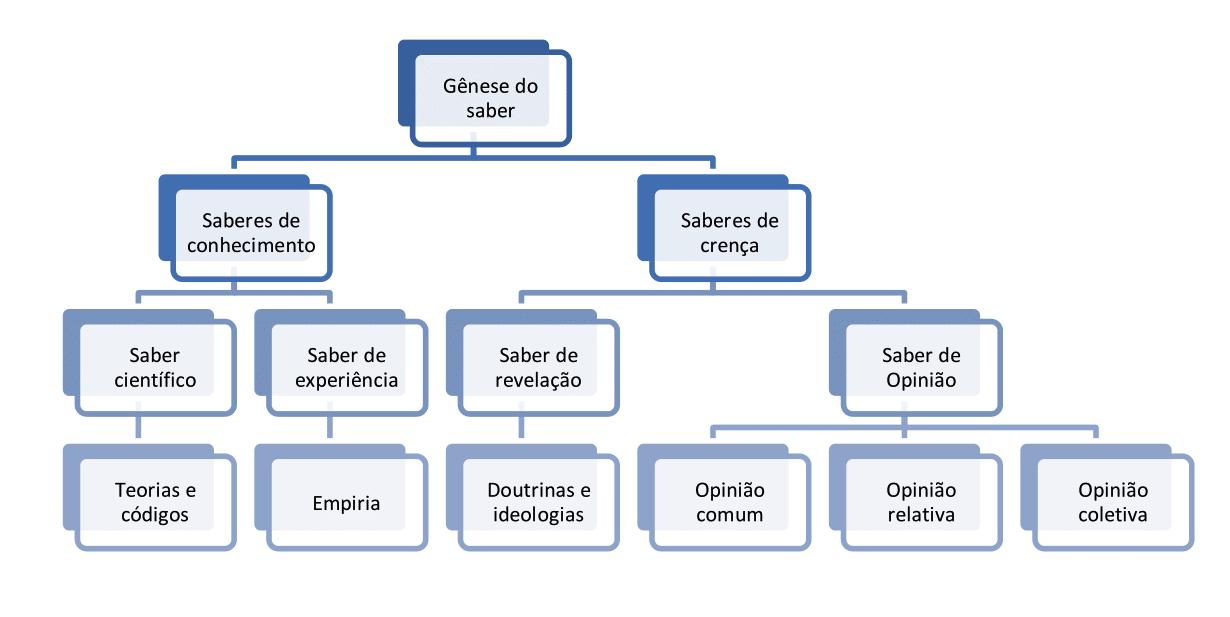
\includegraphics[width=0.8\linewidth]{46657-Outros-142489-163426-2-20230627.png}
    \caption{Diagrama da formação dos imaginários sócio-discursivos.}
    \source{\cite[p. 188]{procopio_os_2009}.}
    \label{fig1}
\end{figure}

Os imaginários sociodiscursivos são engendrados a partir dos vários tipos de saber, como se percebe. Eles fundamentam os discursos que circulam na sociedade e servem de criação dos imaginários e sustentação para a argumentação. São eles que alimentam a ação de construir imaginários, produzindo o sentido social para os eventos que acontecem no mundo. No entanto, mesmo constituindo o mundo, os imaginários, em sua fluidez, dada a natureza do homem e tudo que o cerca, podem ser considerados de perspectiva coletiva ou individual. 

O imaginário coletivo baseia-se em atividades de simbolização inseridas em práticas sociais, tais como artística, religiosa, política, educacional. No que tange ao imaginário individual, percebe-se que ele depende de um julgamento pessoal/íntimo, que se embasa no local no qual o sujeito se insere, mas que se encontra atravessado por outros discursos. Logo, “o imaginário não é nem verdadeiro nem falso”, mas uma proposta de visualização do mundo tangível que se apoia nos saberes, permitindo a construção dos sistemas de pensamento \cite[p. 8]{charaudeau_os_2017}. 

Os imaginários sociodiscursivos que atravessam os discursos dos influenciadores sobre o ensino de escrita da redação do ENEM pautam-se na movimentação destes tipos de saberes descritos anteriormente, visto que o tipo de saber reivindicado  fundamentará o modo de ver e de agir de influenciadores quanto ao ensino da redação do ENEM. Os tipos de saberes são, portanto, noções fundamentais para a compreensão do imaginário sociodiscursivo do ensino de escrita de influenciadores digitais. 

\section{De blogueiros a influenciadores a serviço do mercado}\label{sec-fmt-manuscrito}
Tecnologias Digitais da Informação e Comunicação (TDIC) passaram a definir padrões de interação, assim como práticas de vida nos âmbitos profissionais e pessoais. Espaços e tempo se alongam ou encurtam e, em consequência, alterações na cultura vão se consolidando. 

Na visão de \textcite{karhawi_influenciadores_2017}, é o cenário tecnológico que facilita a interação dos sujeitos na esfera pública por meio da projeção de egos anônimos que se tornam “produtores de conteúdo”. Considerando-se a importância do \textit{ethos} para as trocas simbólicas \cite{maingueneau_proposito_2008} e para a consolidação da imagem de dado influenciador, vemos, então, um cenário em que o influenciador se torna o maior fiador de si mesmo.

Nesse sentido, o público e o privado extinguem as fronteiras, tendo em vista que os inicialmente chamados blogueiros e, atualmente denominados influenciadores, emergem dessa diluição de espaços. O termo blogueiro nasce da ação de se criar um \textit{blog} em que haveria uma lista de \textit{links} sobre assuntos variados ainda no final da década de 1990. \textcite[p. 49]{karhawi_influenciadores_2017} aponta que “os blogueiros da época, \textit{experts} em HTML, atuavam como filtros de conteúdo da rede, disponibilizando comentários e o endereço das páginas que visitavam”. 

Com o passar dos anos, contudo, e com a criação de plataformas como \textit{blogger} e o \textit{Wordpress}, não somente os \textit{experts} alimentariam \textit{blogs}, mas também pessoas comuns. Isso somente tornou-se realidade a partir dos anos 2000, coincidindo com o período de disseminação do uso popular da internet no Brasil e da era da Web 2.0.4 \cite{karhawi_influenciadores_2017}.  \textcite{yunes_representacoes_2019} apontam que essa rápida transmissão de informações implodiu o que se entendia por “real” e “virtual”, favorecendo que o conhecimento cultural e humano fosse distribuído a todos, de certa forma, de maneira democrática. 

Com a entrada desses “novos sujeitos” na sociedade em rede, conceito proposto por \textcite{castells_informationalism_2004}, tudo estaria conectado a partir da divulgação de informações em rede, que não possui centro, apenas nós que podem estar interconectados. À vista disso, os \textit{blogs} passaram a ter uma pessoalidade e a serem utilizados como uma ferramenta de diário pessoal. Logo, há nesses novos \textit{blogs}, a partir dos anos 2000, uma marcação de identidade, voz e autoria, dando início a cultura da participação \cite{karhawi_influenciadores_2017}. 

Entende-se hoje que o blog é um gênero centralizado na figura de um blogueiro, que é uma pessoa famosa ou não na comunicação, que se interconecta a outros \textit{blogs} de um mesmo seguimento, definindo a chamada blogosfera. Essas pessoas são vistas como veículos de informação e possuem uma credibilidade construída pelo mercado econômico a partir dos discursos que proferem e da imagem de si que estabilizam. Nesse sentido, tem-se os \textit{blogs} temáticos, que possuem como porta voz um sujeito, antes anônimo, que realizava alguma tarefa, e que agora repassa dado conhecimento em larga escala de público \cite{karhawi_influenciadores_2017}.

Os \textit{blogs} cedem espaço gradativo para redes sociais a partir da primeira década dos anos 2000. E as redes passam a ocupar um tempo cada vez maior na vida de seus usuários, permitindo perceber quão importante é para o usuário acessar conteúdos de maneira recorrente. Esse tempo usado em redes sociais como \textit{Instagram}, \textit{TikTok} e \textit{Youtube} aproxima os consumidores de conteúdo dos produtores, deixando uma imagem de que são verdadeiramente próximos e íntimos, favorecendo a adesão ao discurso influenciador \cite{yunes_representacoes_2019}. \textcite[p. 37]{castells_internet_2002} revela que “a cultura da internet acontece a partir dos seus criadores, que através de uma lógica de valores e crenças influenciam os comportamentos dos produtores/usuários que estão imersos neste sistema cultural”. 

Com o avanço das mídias viu-se então a possibilidade de inserção do audiovisual em plataformas digitais e, nesse contexto, em 2005, foi criado o \textit{Youtube}, com o objetivo de ser uma plataforma que alocasse vídeos de grande porte e que pudessem ser vistos por muitas pessoas. Com isso, o slogan da plataforma, que é “transmita-se”, em português, evidencia o convite a todos os sujeitos a sair de um lugar de anonimato para um lugar de destaque na internet. Cabe salientar que nesse período o termo influenciador digital ainda não havia sido utilizado, tendo em vista que as primeiras publicações no \textit{YouTube} no Brasil estão datadas do ano de 2010. Então, os termos utilizados eram “videoblogueiro” e “vlogger” e, mais recentemente, “\textit{Youtuber}” \cite{karhawi_influenciadores_2017}.

A partir de 2011, como aponta \textcite{karhawi_influenciadores_2017}, houve um processo de monetização da prática de postar vídeos, consolidando o termo “\textit{Youtuber}” como profissão. Isso foi bem aproveitado pela indústria, visto que agora haveria outras possibilidades de divulgação de produtos para um público específico, de acordo o nicho do \textit{Youtuber}. Dessa maneira, a influência já aparece de modo velado na escolha da indústria para a divulgação do seu produto, contudo percebe-se que o termo “formadores de opinião” só apareceu a partir do ano de 2011 na mídia tradicional \cite{karhawi_influenciadores_2017}.

Enquanto participantes do processo de comunicacional interacional, todos estão sujeitos a sofrerem influência, seja da família, seja da escola, seja dos meios de comunicação como um todo, assim como estão sujeitos a exercer influência, como ressalta \textcite{azevedo_agendamento_2004}.

Atualmente, é notório que o chamado influenciador, enquanto formador de opinião, além de ser alguém que apresenta dadas credenciais de confiabilidade na visão do público, é ainda uma figura que se alicerça na atividade de curadoria, pois é concebida também como um repassador, visto que ele consome o que é veiculado na mídia e, posteriormente, repassa o que foi consumido, tratando o conhecimento e selecionando o que seu público provavelmente gostaria de consumir. É a lógica da oferta e do consumo.  

\textcite{karhawi_influenciadores_2017} classifica os influenciadores digitais em verticais ou horizontais. O vertical possui uma credibilidade já instaurada em um grande público, visto que tem “crédito” por ser previamente conhecido. Além disso, detém a capacidade de inserir valores, ideias e ideologias ligadas à sua imagem sem empecilhos, podendo ser definido como “intelectuais, jornalistas, professores, líderes de classes, empresários, lideranças comunitárias” \cite[p. 52]{karhawi_influenciadores_2017}. O horizontal não possui imagem de credibilidade prévia, todavia possui um traço de personalidade característico, que é utilizado como ferramenta de adesão aos seus discursos, podendo ser traços de liderança, por exemplo. Sendo assim, qualquer pessoa pode se ocupar deste posto de formador de opinião horizontal, podendo ser professores, médicos ou apenas pessoas comuns \cite{karhawi_influenciadores_2017,resende_professores_2020}. 

Na era digital o formador de opinião passa a ser chamado de \textit{influenciador digital} (\textit{digital influencer}); é aquele que vai comercializar seu saber e sua opinião, alocando-os em plataformas digitais e lucrando a partir do número de seguidores, \textit{likes} e visualizações. Eles possuem o protagonismo na transmissão de informações pela via da cibercultura e influenciam na disseminação de assuntos que, para este estudo, inclui a esfera educacional.

A influência no campo educacional ocorre devido ao estímulo constante por meio da disseminação de saberes que levam os educandos a se perceberem como sujeitos ativos no processo de aprender. Assim, a mercadoria oferecida é justamente o conhecimento, embora muitas vezes simplificado ou objetificado por meio certo pragmatismo imediatista.

A intensa cultura digital de nossos tempos desempenha uma função instrumentalizadora para a disseminação da cultura. Como agentes de uma indústria cultural \cite{adorno_dialetica_1985} que cria e fortalece valores retroalimentando-os, influenciadores digitais educacionais ofertam conteúdos escolares como mercadorias a serem adquiridas por meio do consumo constante de “pílulas de conhecimento” (pequenas porções de conhecimento simplificado) oferecidas por dado influenciador. 

Nesse contexto, a Indústria Cultural retira do tipo horizontal de formadores de opinião as pessoas comuns e as leva para um lugar de destaque no âmbito da comunicação de massa, ou seja, essas pessoas tornam-se celebridades (influenciadores verticais) que, muitas vezes, não compartilham apenas saberes ou opiniões, mas também o seu dia a dia, que se torna digno de admiração. Nesse sentido, a influência passa a exercer sua função em diferentes campos, tais como o ideológico, político, social e comercial \cite{resende_professores_2020}.

Influenciadores digitais parecem estar, então, num limbo entre influenciadores verticais e horizontais. Embora muitos tenham entrado neste mercado numa perspectiva horizontal, ganharam fama e, hoje, são vistos como pessoas com credibilidade pregressa, embora construída no exercício da atividade \cite{resende_professores_2020}.  Esse cenário de mudança entre os sujeitos também impactou os professores, que se viram cada vez mais imbuídos de ocuparem esse espaço de influência digital, seja para fins educacionais, seja para fins profissionais e econômicos. 

Com a pandemia de COVID-19, observou-se que houve um aumento exponencial de canais no \textit{YouTube}\footnote{A afirmação baseia-se em dados disponibilizados pela plataforma do Centro Regional de Estudos para o Desenvolvimento da Sociedade da Informação (CETIC.BR), disponível no site:  \url{https://www.cgi.br/publicacao/painel-tic-covid-19-pesquisa-sobre-o-uso-da-internet-no-brasil-durante-a-pandemia-do-novo-coronavirus-3-edicao/}.} com a finalidade educacional, principalmente porque foi um período em que a escola experimentou um novo formato, em que professores e alunos tiveram que adequar suas práticas. Desse modo, muitos canais intitulados como “Edutuber”\footnote{Canais no Youtube inseridos no nicho educacional. Educação + \textit{Youtuber}= Edutuber.} surgiram a fim de contribuir com a nação em um momento de crise sanitária, como atesta a propaganda dos próprios canais.

Todavia, para além da crise sanitária, também foi um momento propício para aumentar o retorno financeiro, visto que a demanda estava em alta e poucos canais falavam sobre assuntos educacionais de maneira tão direcionada. Desse modo, interesses de monetização estão, obviamente, acima da preocupação com a nação.

É possível remontar à teoria Crítica de \textcite{adorno_dialetica_1985} para perceber que a Indústria Cultural transforma o que seria conhecimento em mais uma mercadoria cultural, tendo em vista que os discursos são pautados na lógica mercadológica vigente: o lucro por meio das visualizações, a disseminação de uma imagem, a oferta de saberes desejáveis em forma e conteúdo prontos para o consumo. Portanto, a influência é exercida para monetização, servindo à lógica vigente da capitalização de serviços. Este ponto precisa ficar claro para se compreender aspectos do discurso dos influenciadores, como o apelo à exclusividade do modelo de ensino que oferecem, elemento comum nas relações.


\section{Procedimentos metodológicos}\label{sec-formato}
Este estudo assume uma metodologia qualitativa e uma perspectiva interpretativista. Para delinear os imaginários sociodiscursivos do ensino da redação do Enem de influenciadores digitais, foram selecionados três vídeos de influenciadores que focalizam a elaboração da redação do Enem em seus canais do \textit{Youtube}. 

A seleção de vídeos ocorreu por meio de um recorte temático, temporal e quantitativo: para o primeiro aspecto os termos de busca foram “redação + Enem”; para o segundo, foram delimitados vídeos postados em 2020 e 2021 e, para o terceiro, o foco esteve no maior número de visualizações na época da busca\footnote{A busca foi realizada no mês de fevereiro de 2022.}. Assim, chegou-se à seleção dos primeiros vídeos que apareceram na listagem da plataforma (os mais visualizados) com os filtros adicionados, como indica a \Cref{tbl1} seguir:

\begin{table}[htbp]
\centering
\small
\begin{threeparttable}
\caption{Vídeos selecionados.}
\label{tbl1}
\begin{tabular}{p{2.5cm} p{3.5cm} p{3.5cm} p{3.5cm}}
\toprule
\multirow{2}{*}{Título do Vídeo} & Vídeo 1 & Vídeo 2 & Vídeo 3  \\
& A verdadeira estrutura da Redação Enem & Meu modelo de redação nota 1000 para Enem 2021 & Revisão de redação para o Enem 2020 + dica de vestibular online! \\
\arrayrulecolor[gray]{.7}
\midrule
Duração em minutos & Nove minutos e vinte e seis segundos & Dezoito minutos e cinquenta e três segundos & Dezessete minutos e trinta e cinco segundos \\
\midrule
Número de visualizações & 171.179 & 534.271 & 237.826 \\
\midrule
Canal & Professor Noslen & Felipe Araújo & Débora Aladim \\
\midrule
Biografia do Influenciador & Noslen Borges de Oliveira é professor de Língua Portuguesa há mais de 17 anos. Já atuou em Universidades à distância como tutor. Já lançou livro sobre o ensino de gramática e é dono do maior canal de ensino de Língua Portuguesa do YouTubeMundial & Felipe Araújo é formado em Odontologia e se diz um produto da educação, pois foi através dela que ele ascendeu socialmente. Ele começou a estudar sozinho, pois não tinha onde estudar ou dinheiro para custear algum curso e, a partir dos estudos, elaborou metodologias e hoje as compartilha no YouTubee vende seus cursos em sua plataforma. & Graduada em História pela Universidade Federal de Minas Gerias, Débora Aladim começou a gravar conteúdos para o YouTube desde 2013. Ela despontou na plataforma após revelar seu método de escrita e hoje conta com uma plataforma em que vende seus cursos voltados para o ensino de redação e história. \\
\midrule
Breve resumo do vídeo & O vídeo tem como objetivo ensinar os alunos, na véspera do ENEM, como escrever uma dissertação argumentativa. Ele inicia dizendo o que é dissertar. Segundo ele é se aprofundar sobre os temas, ou seja, sair do senso comum. Logo, é necessário saber o como (estrutura), que é o ponto central do vídeo. Por fim, ele discorre sobre as habilidades para se escrever uma boa redação.  & O influenciador inicia o vídeo abordando que o modelo de escrita é um suporte aos alunos, para que eles otimizem o tempo de prova. Contudo ele ressalta que é necessário compreender a estratégia e que isso é possível por meio do canal dele, através da visualização de outros vídeos. Após isso ele apresenta os parágrafos, exemplificando sobre cada ponto.  & O canal da Débora Aladim inicialmente foi criado com o intuito de propagar conteúdos sobre História. Atualmente ela é graduada nesta área, mas seu canal também aborda sobre temas relacionados à elaboração da redação modelo Enem. O vídeo analisado serve como propaganda para o “Quero Bolsa” e viabiliza de maneira sintetizada o passo a passo de como escrever uma boa redação. \\
\midrule
\emph{Link} de acesso & \url{https://www.youtube.com/watch?v=jN1PzHGxom0} & \url{https://www.youtube.com/watch?v=SCnd-ynVNnA} & \url{https://www.youtube.com/watch?v=U1oFBNabLcg} \\
\arrayrulecolor{black}
\bottomrule
\end{tabular}
\source{Elaboração própria.}
\end{threeparttable}
\end{table}

Por meio de uma análise panorâmica dos dados foi possível identificar quatro categorias macrotemáticas nos dados: i) a projeção de uma modelagem textual pessoal; ii) a projeção e a resolução de dificuldades dos estudantes; iii) esquematização/modelização do ato de escrever iv) ensino de escrita como mercadoria cultural. A seguir, discorre-se sobre cada uma delas.

\section{O tecer dos imaginários sobre o ensino de escrita: uma análise dos discursos dos influenciadores digitais}\label{sec-modelo}
O ensino de escrita, na visão de influenciadores digitais, parte de alguns pontos essenciais a serem analisados nos trechos do \textit{corpus} transcrito. À vista disso, organizamos a análise de maneira intercalada, a fim de que o delineamento dos imaginários seja processual e multifacetado. 

\subsection{A projeção de uma modelagem textual pessoal }\label{sec-organizacao}
Inicialmente, observa-se, a partir da análise das transcrições dos vídeos, que os influenciadores digitais se pautam em discursos que transformam o processo de escrita em um saber que foi experienciado por eles. Trata-se, portanto, nesse caso, de um saber de experiência que é (re)constituído, baseando-se nas competências da redação do Enem. Tal afirmativa pode ser visualizada a partir dos seguintes trechos: 

\begin{quote}
    01. Hoje a gente vai ter uma revisão do meu método de como escrever redação modelo Enem. Passo a passo para você ficar preparadinho e confiante também no dia da prova. (Débora Aladim)
\end{quote}

\begin{quote}
    02. No vídeo de hoje eu vou apresentar o modelo de redação que eu desenvolvi para o Enem 2021. Modelo totalmente validado que se encaixa em qualquer tema e que tem os componentes necessários para uma nota mil, beleza? Então pega um papel, uma caneta e vamos ‘'simbora''conhecer ele. (Felipe Araújo)
\end{quote}

\begin{quote}
    03. Éa hora de nós descobrirmos como funciona essa estrutura da redação do Enem [ao fundo aparece: A verdadeira estrutura da redação do Enem] Dissertação-argumentativa daquele jeitão que eu já te falei. Daquele jeitão bonitão, que é o que? Aquilo que tem na minha plataforma. Plataforma? Sim! www.professornoslen.com.br e eu tô entregando para você. Assim, com todo amor e carinho. Bora para aula?(Professor Noslen).
\end{quote}

A utilização de pronomes possessivos na apresentação da estrutura prototípica da redação do Enem – \textit{meu método} (01); \textit{eu desenvolvi} (02), \textit{minha plataforma} (03) – revela um saber de conhecimento visto como pessoal que é utilizado como mecanismo de embasamento de uma experiência bem-sucedida e particular, portanto, exclusiva e não generalizada.

Esse saber de experiência é validado a partir da aderência dos estudantes ao discurso de sucesso do influenciador. Contudo, como veremos a seguir, no trecho 04, o influenciador Felipe Araújo valida seu discurso não somente pelo seu sucesso obtido no Enem, mas também através de saberes de conhecimento sobre o processo de ensino de escrita, pautado no que foi divulgado pelo Instituto Nacional de Estudos e Pesquisas Educacionais Anísio Teixeira (INEP) no ano de 2020, através das cartilhas dos corretores. 

\begin{quote}
    04. Esse modelo que eu vou apresentar para vocês agora foi construído totalmente em cima dessas cinco competências, tendo como principal suporte o manual de correção da redação. O material inédito que foi disponibilizado pela INEP pela primeira vez no ano passado (2020) e que detalha cada uma das cinco competências, beleza? Então bora lá! Primeiramente, é importante que a gente saiba que a redação do Enem é escrita em um formato de texto chamado de dissertativo-argumentativo (Felipe Araújo).
\end{quote}

Este quadro de oscilação entre os tipos de saberes coaduna com o pensamento de \textcite[p. 16]{charaudeau_conquista_2020}, que diz que “o saber precisa ser complementado pelo saber-fazer. Entretanto, pode-se ter a competência de saber-fazer sem necessariamente possuir conhecimentos”. Dessa maneira, a autoridade dos influenciadores digitais pode então ser construída a partir da experiência do sujeito que “está” professor de redação - como é o caso de dois dos influenciadores analisados (Débora Aladim e Felipe Araújo) - que não se autointitulam em seus vídeos como professores, como Noslem o faz. Apesar disso, o trecho 04 também demonstra que o sujeito se apoia no “discurso oficial” sobre a prova, lançando mão das instruções do INEP, certamente para somar à sua experiência o efeito de autoridade do discurso oficial. 

\textcite{charaudeau_conquista_2020} aponta que o saber-fazer pode ser adquirido não apenas pela necessidade técnica e pela exigência conceitual, mas também pela prática contínua da mesma atividade. Logo, o que se observa pelos trechos em tela e pela biografia dos sujeitos é que, nos casos do influenciador Felipe Araújo e de Débora Aladim, o conhecimento foi adquirido pelo exercício da experiência, pois ambos não têm formação na área em que atuam no canal na plataforma Youtube. 

A experiência comprovada pelos influenciadores se dá partir dos seus resultados particulares, aprovações em vestibulares, número de visualizações e de inscritos no canal. Demonstram, portanto, saber-fazer, isto é, possuir a competência para tal e, por consequência, poder ensinar.

Esse saber de experiência revelado a partir dos discursos dos influenciadores se cristaliza à medida que a imagem que veiculam os associa categoricamente à verdade, construindo uma espécie de saber de revelação.

\subsection{A projeção e a resolução de dificuldades dos estudantes}\label{sec-organizacao-latex}
Outro tipo de saber mobilizado pelos influenciadores durante os discursos é referente ao saber de crença, que se baseia no saber de opinião relativa, que se pauta na visão individual ou coletiva, atribuindo valor sobre pessoa ou situação. Nesse caso, observa-se nas falas que os influenciadores se colocam como aqueles que podem antecipar dificuldades, num processo de interação com a audiência:

\begin{quote}
   05. Se tu não sabe nada de redação do Enem, decora modelo e utiliza ele lá no dia da prova, grandes são as chances que tu se perca. Eu falo isso, porque lá no dia da prova tu vai precisar pegar aquela estrutura e fazer com que ela se adeque aquele tema da redação. E sem conhecimento pessoal, vocês vão fazer isso de jeito nenhum (Felipe Araújo).
\end{quote}

\begin{quote}
  06. Eu sei que uma dificuldade que muita gente tem é como começar a redação, né!? Geralmente as primeiras linhas são as mais difíceis, porque é quando você precisa, né, colocar a mão na massa e tudo mais. Uma dica muito boa para você começar é já começar a citando outra área. Às vezes falar de um livro, de um filme, falar de outro país, comparar o Brasil com algum outro país, uma alusão histórica, uma frase de filósofo (Débora Aladim).
\end{quote}

\begin{quote}
  07. E chegou a redação que todo mundo espera. Sim! Dissertação-argumentativa. Todo mundo espera por quê? Porque é mais cobrada na face da terra, do universo, Brasil, Europa, Portugal. Não, Brasil. Certo? Olha só, a dissertação argumentativa é o gênero mais cobrado no Brasil em vestibular, Enem, concurso, todas as provas que têm algum tipo de concurso é a dissertação argumentativa. Óbvio que existem alguns vestibulares do Brasil que cobram outros gêneros, mas essa é mais recorrente (Professor Noslen). 
\end{quote}

O saber de opinião relativa atribui uma percepção dos influenciadores sobre o que os estudantes consideram “dificuldades”. Os influenciadores se colocam como conhecedores das dificuldades alheias e, nesse sentido, como aqueles capazes de saná-las. O influenciador Felipe Araújo, no trecho (05), diz que a falta de conhecimentos gerais dos estudantes levará ao insucesso na repetição do modelo proposto por ele. Já a influenciadora Débora Aladim considera como dificuldade \textit{de muita gente} (06) começar a escrever a redação e indica uma solução para isso: citar conhecimentos gerais. Por último, no trecho (07), o influenciador Noslen considera a dissertação-argumentativa como a\textit{ mais cobrada na face da terra}, o que viabiliza a abordagem constante do assunto em seu canal. 

A partir desse trecho, observa-se que há uma valoração atribuída pelos influenciadores que reforça a ideia de proximidade entre eles e os anseios de qualquer estudante que realiza um processo seletivo: passar com uma boa nota e conseguir a vaga no curso almejado. Desse modo, o argumento de validação da relevância do seu conteúdo revela uma empatia e proximidade entre o que o influenciador oferece e o que o estudante necessita, delineando o imaginário de que ensinar a escrever é identificar dificuldades para diminui-las. 

Logo, o influenciador coloca em voga um \textit{ethos} que se expressa pela empatia pelos estudantes e pela compreensão de suas dificuldades, pois o influenciador pode também ter partido de um lugar de anonimato, o que facilita a aproximação, pois tanto o gerador de conteúdo, inicialmente, quanto o estudante são pessoas comuns que, nesse caso, passaram por situações comuns: a realização da escrita da redação do Enem.

\subsection{Esquematização/modelização do ato de escrever}\label{sec-titulo}
Observou-se ainda no \textit{corpus} a movimentação mútua de saberes de crença e saberes de conhecimento que vão validar a perspectiva de texto prototípico a ser internalizado pelo aluno: o modelo de redação Enem é apresentado como um esquema a ser preenchido. Palavras como: “modelo”, “a verdadeira redação do Enem”, “Passo a passo”, “frases prontas” e “estrutura pronta” se fazem recorrentes no discurso dos influenciadores, o que acaba por esvaziar discursos teóricos que veem o processo de escrita como uma construção do sujeito a partir do seu envolvimento com a linguagem. 

Como exemplo, nota-se que os influenciadores se utilizam de saberes de conhecimento para fechar as possibilidades de utilização de escrita pelos estudantes: 

\begin{quote}
  08. Não adianta você simplesmente jogar os argumentos lá, você tem que selecionar, você tem que ir né!? Usar linguagem a seu favor... Nesse caso eles exigem que você tenha seis conectivos na sua redação, mas eu vou explicar isso melhor mais tarde (Débora Aladim).
\end{quote}

A influenciadora, ao utilizar o pronome eles, delega a responsabilidade de exigência do uso de conectivos a uma “instância superior”, talvez tida como pouco acessível aos estudantes, mas certamente acessível aos influenciadores, embora a validação venha da própria cartilha do Enem. Nota-se que a exigência quantitativa feita por “eles”, nesse caso, o Enem, também pode ser percebida no discurso de Felipe Araújo, no trecho 04. 

Ao validar seu discurso a partir de competências requeridas pela prova (como o uso de conectivos), movimenta-se uma espécie de saber de conhecimento científico (tido como verdade), visto que o ensino está baseado na cartilha disponibilizada pelo INEP (por extenso na primeira vez) para a formação dos corretores, indicando que o texto, de acordo com o próprio discurso oficial, deve ser “formatado” a partir de certos critérios. Há, então, parâmetros a serem seguidos para que o texto esteja dentro da expectativa do padrão de correção da cartilha. Em complemento, os discursos dos influenciadores também utilizam o saber de conhecimento de experiência, como vimos, revelando que eles detêm a estrutura padronizada, e que ela é passível de ser “copiada”, uma vez que é justamente isso que os influenciadores buscam ensinar. 

Logo, percebe-se que o estudante não precisa compreender metacognitivamente o seu processo de escrita, como teóricos da linguagem postulam (saber de conhecimento científico), mas sim conseguir reproduzir o modelo que os influenciadores repassam em seus vídeos, porque eles foram validados, ou seja, obtiveram uma boa nota no Enem, e/ou a razão dos seus alunos obterem êxito (saber de experiência). Os trechos a seguir ilustram essa visão:

\begin{quote}
  09. Então vamos lá, pessoal! Passo a passo o que cada parágrafo tem que ter. Meu método usa quatro parágrafos na redação: o primeiro parágrafo vai ser o parágrafo de introdução. Nesse parágrafo você tem que fazer duas coisas: você tem que contextualizar e problematizar (Débora Aladim)
\end{quote}

\begin{quote}
  10. Vocês estão entendendo? A minha forma de argumentar é essa justamente porque o nosso último parágrafo, que a proposta de intervenção é quando a gente vai resolver esses problemas. Então você vai fazer o texto que conversa muito entre si, né? Você começa falando que existe uma situação problemática no Brasil, você explica porque que ela é um problema, depois porque que esse problema ainda não foi resolvido e depois você resolve o problema. Então essa é a minha forma de escrever. (Débora Aladim)
\end{quote}

A postura revelada a partir dos discursos dos influenciadores nos excertos 09 e 10 é individualista, visto que o saber de conhecimento (acessível a todos) apresenta-se em detrimento do saber de experiência (próprio a alguns) que está sendo valorizado pelos influenciadores. Tal postura é revelada no ato de conceber o ensino de escrita como um método pessoal - \textit{o modelo de redação que eu desenvolvi} (02), \textit{meu método usa quatro parágrafos na redação} (09), \textit{a minha forma de argumentar} (10).

O saber de experiência explica o processo de escrita a partir dos moldes criados pelos influenciadores. Coloca-se, aqui, a partir de um \textit{ethos} de sucesso no Enem, um parâmetro de modelo de escrita a ser copiado pelos estudantes que consomem esse conteúdo. Desse modo, percebe-se que ainda que se mencione saberes de conhecimento científico, estes não se sobrepõem aos saberes de experiência, tendo em vista que a forma como os influenciadores estruturam a redação modelo Enem é pautada sobretudo no sucesso pessoal.

Nota-se, portanto, que o próprio Enem, enquanto política pública de acesso ao Ensino Superior, reforça a produção destes modelos transformados em produtos educacionais, neste caso os cursos de ensino de escrita que se pautam em prototipicidade e não em um ensino metacognitivo. O molde, a redação perfeita, isto é, nota mil, deve seguir rigorosos padrões para se intitularem desta forma. 

\subsection{Esquematização/modelização do ato de escrever}\label{sec-autores}
O argumento do produto exclusivo, a esquematização fácil e a resolução de problemas por antecipação estabelecem claramente uma relação de comércio em que a mercadoria cultural é o ensino da escrita da redação Enem, visto que tal ensino se torna uma mercadoria à medida que o próprio sistema reforça a padronização do texto. Nos trechos a seguir é possível flagrar momentos da relação mencionada. 

\begin{quote}
  11. Antes mesmo de começar já tenho uma dica incrível para você treinar, que é o vestibular premiado Quero Bolsa. Para quem não conhece é uma prova 100\% gratuita, 100\% online e que dá bolsa de 100\%. A prova já está disponível e vai ficar até o dia 29/01, você pode fazer no dia e na hora que for melhor para você. Não precisa agendar é só entrar no site deles, o link vai estar aqui na inscrição e fazer a prova. 
  
Vale muito a pena conferir, gente! É uma oportunidade incrível! Você faz a prova no dia e na hora que for melhor para você. Vai estar disponível até o final do mês, vou deixar o primeiro linkna descrição e esse ano vai fazer, inclusive, três anos que eu trabalho com o Quero Bolsa. Sou apaixonada por eles, vocês bem já sabem. Então não deixem essa oportunidade passar, tenho certeza que vai ajudar muito! (Débora Aladim).
\end{quote}

\begin{quote}
  12. E não esquece! Se inscreve aqui no canal, sempre se inscreve porque se inscrevendo você me ajuda muito a poder continuar produzindo “de edu” ou “dinheiro”, digo, produzindo de educação não, continuar produzindo conteúdo de educação para você que está aqui junto comigo no canal. Maravilha? Então se inscreva no canal agora, já deixe seu comentário se você está curtindo esse tipo de aula.  Tchau e até a próxima! Valeu! Fui! (Professor Noslen).
\end{quote}

\begin{quote}
 13. Felizmente, aqui no canal tem vídeos pra tu sair doutor em redação. Então, se tu é inscrito aqui no canal, com certeza absoluta isso é não é um problema para ti (Felipe Araújo).
\end{quote}

Os discursos analisados revelam que se ensina redação como se vende um produto, todavia a cena enunciativa revela que a preocupação não é apenas ensinar a escrita da redação: há algo mais em comércio, que pode ser tanto a imagem de si quanto produtos educacionais distintos (como o Quero bolsa). 

O estudante “consumidor” desses conteúdos espera justamente a aprovação no vestibular. Desse modo, ao ofertar a possibilidade de um vestibular que o retire desta condição de vestibulando, a influenciadora Débora Aladim, no trecho 11, utiliza-se de seu poder de influência sobre os estudantes para apresentar abertamente o objetivo de levar o seu público a consumir produto ou serviço. Dessa maneira, o \textit{ethos} de sucesso na escrita, construído por esses influenciadores digitais, baseia-se na essência da definição de formadores de opinião, o que permite uma adesão sem maiores críticas por parte dos estudantes. 

Já no trecho 12, o influenciador Noslen profere um ato falho, revelando que na verdade o que se produz é dinheiro em primeiro plano.  Por fim, o trecho 13 argumenta que atingir a formação educacional completa é muito fácil, basta estar inscrito no canal do influenciador Felipe Araújo que isso será possível. Logo, observa-se uma banalização da formação educacional comprometida com processos de desenvolvimento orientados à emancipação e autonomia. 

As análises dos vídeos demonstram que os saberes de conhecimento (científico e de experiência) movimentados nos vídeos se sobrepõem, pois para embasar uma experiência pautada na empiria, os influenciadores utilizam-se da teoria e dos códigos do INEP para validar um saber-fazer empírico e gerar adesão. Com isso, essa sobreposição também se utiliza de maneira concomitante do saber de opinião, revelando o imaginário de que a redação nota máxima do Enem é aquela que segue passos predeterminados, esvaziando a escrita como um processo de interlocução e interação mediada pela linguagem, como aponta a função da linguagem como recurso de interação social. 

As análises, portanto, demonstram que o imaginário sociodiscursivo que alicerça o ensino de escrita da redação do Enem alia saberes de conhecimento com saberes de crença (com predomínio do primeiro, mais especificamente do saber de experiência) na compreensão desse fazer por meio: i) da projeção de uma modelagem textual considerada pessoal; ii) da capacidade de antecipação de dificuldades dos estudantes para a consequente oferta de soluções; iii) da disponibilização de uma esquematização formulaica a ser reproduzida iv) do ensino de escrita como mercadoria cultural pronta para consumo imediato.

\section{Conclusão}
Os vídeos que compõem o \textit{corpus} veiculam discursos que afastam os alunos de uma consciência sociocomunicativa da linguagem, pois apresentam modelos simplificados a serem seguidos. O capital cultural aqui concebido como o processo de ensino-aprendizagem de escrita é tido como uma receita tanto pelos influenciadores quanto pelo próprio INEP, que formata cada vez mais ao longo dos anos o modelo de correção e, com isso, escrita dos estudantes brasileiros. 

O interesse em fazer com que os estudantes se alienem de um saber metacognitivo sobre a escrita, que não pensem criticamente e que se apoiem em fórmulas rápidas, no fundo, parece ser do próprio Estado, representado pelo Enem e pelo INEP. Ao permitir que o mesmo gênero textual componha a prova por mais de duas décadas e ao engessar gradativamente o processo de correção dos textos, o Estado produz uma visão de educação linguística que serve aos seus interesses. Dessa maneira, os influenciadores são percebidos como meros propagadores de discursos que o aparato ideológico do estado engendra.

Por fim, o imaginário somente reforça a ideia de que a reprodução se dá em todos os âmbitos e que o processo de ensino de escrita voltado para o Enem precisa ser repensado urgentemente, visto que estamos repetindo erros cometidos desde a década de 1960 com o método retórico-lógico. 

\printbibliography\label{sec-bib}

\begin{contributors}[sec-contributors]
 		\authorcontribution{Lilian Karla Rocha}[conceptualization,datacuration,formalanalysis,investigation,methodology,writing]
 		\authorcontribution{Maria Clara Maciel de Araújo Ribeiro }[conceptualization,datacuration,formalanalysis,projadm,review]
\end{contributors}

\end{document}
